\noindent The \ac{sm} of Particle Physics is the current theory that describes three of the four fundamental forces, namely the electromagnetic, strong, and weak forces, with the exception of gravity. Over the last decades it has been probed with remarkable precision but although there are  observational phenomena that lie beyond its scope.

The SM is based on symmetry principles and is described by a lorentz-invariant \ac{qft} that is renormalizable and invariant under local gauge transformations. This means that within the non-abelian gauge group
\begin{equation}
    G = SU(3)_C \otimes SU(2)_L \otimes U(1)_Y,
\end{equation}
the equations of motions are invariant. $SU(3)_C$ is the special unitary group of rank 3 representing the color symmetry within \ac{qcd}, the \ac{qft} describing the strong interactions. $SU(2)_L \otimes U(1)_Y$ exhibits the unification of the weak and electromagnetic interaction into the electro-weak force of $SU(2)_L$ left-chiral fermions of the weak force and right-handed $U(1)_Y$ fermions with hypercharge $Y$ of the electromagnetic force described by Quantum Electrodynamics \ac{qed}.

The following describes the particles of the \ac{sm} and gives a brief overview of the \ac{qft}'s used to describe aforementioned forces. The content of this chapter draws inspiration primarily from \citep{hollik2010quantum,griffiths2020introduction,thomson2013modern,zee2010quantum}. Natural units are assumed everywhere $\hbar=c=1$.


\section{Particles of the Standard Model}

All currently known elementary particles are included in the \ac{sm} and can be organized as depicted in figure \ref{fig:sm}. This includes 12 fermions, that are particles of half-integer spin, 12 vector bosons with spin 1, and the Higgs boson, a scalar particle with spin 0.


\begin{figure}
    \centering
    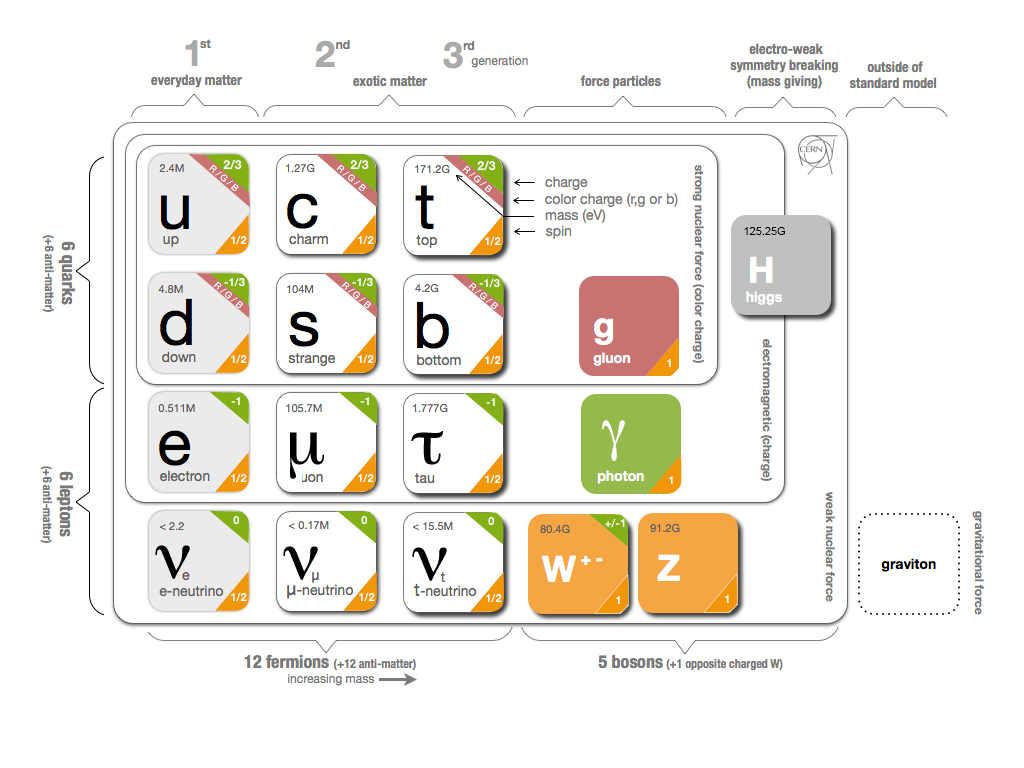
\includegraphics[width=1\textwidth]{SMinfographic_image_}
    \caption[]{Particles in the SM. Adopted from \citep{smpar}. Higgs Boson mass corrected to the current value \citep{particle2022review}. }
    \label{fig:sm}
\end{figure}


The fermions can be categorized into three generations each consisting of a charged lepton, a neutral neutrino and two quarks. Except for their masses, particles of the different generations have the same quantum numbers. Ordinary matter consists only of particles from the first generation. Moreover each particle has an associated anti-particle with all the quantum numbers inversed.

Quarks possess both electric charges and color charges, causing them to interact with each other via weak, electromagnetic, and strong forces. Each generation consists of an up quark (up, charm and top quark) with an electric charge of \mbox{Q = 2/3} and a down quark (down, strange and bottom quark) with a charge of \mbox{Q = -1/3}. Quarks can only be observed as composite particles - hadrons due to color confinement. This states that if one tries to separate a hadron, it is always energetically favorable to produce a quark-antiquark pair instead. Hadrons constitutes either bound states of 2 quarks - Mesons, e.g. a pion or 3 quarks - Baryons e.g. the proton. To not break Pauli's exclusion principle quarks in a bound state must have different color states.

Leptons in turn do not carry a color charge and encompasses the electron $e$, muon $\mu$ and tau $\tau$ and their associated neutrinos $\nu_e$, $\nu_\mu$ and $\nu_\tau$. In the \ac{sm} neutrinos are considered to be massless. Neutrinos also do not carry a charge and interact solely via the weak force whereas the  ones ($e$, $\mu$, $\tau$) with a charge $Q=-1$ participate also interact electromagnetically.

In the interaction picture of \ac{qft}, forces are mediated by particles specific to the particular force. These particles are bosons and are mediating as 8 massless gluons $g$ the strong force, as 1 massless photon $\gamma$ the electromagnetic force and as 3 massive bosons $W^+,W^-,Z$ the weak force.

The scalar Higgs particle has a unique role in the Standard model. A locally gauge invariant \ac{qft} requires massless mediators which the $W^{\pm},Z$ are not. When unifying the weak force and the electromagnetic force into the electroweak force a new field - the Higgs field - can incorporate mass to these mediators by leaving the qft gauge invariant. This will be discussed in detail in section \ref{sec:higgs_mechanism}. The Higgs field can explain the masses of all fermions as the coupling to each fermion is proportional to its mass. This essentially means that the heavier the particle, the stronger its interaction is with the Higgs field.

If not further specified the following always includes the anti-particles when referred to a species or a particular particle.

\section{Quantum Field Theory}\label{sec:qft}
Elementary Particles can be created, transformed and vanish in all sorts of particle interactions. Quantum mechanics states that energy can vary greatly on short time scales via the uncertainty principle. Special relativity relates energy with mass allowing energy to manifest as massive particles. Though special relativity lacks a quantum mechanical description and in non-relativistic quantum mechanics the particle number is conserved. Neither of these descriptions is sufficient to fully describe the observations therefore \ac{qft} was developed.

For a field description some quantity $\phi(x,y,z,t)=\phi(x)$ is assigned to some region in spacetime $x$. Similar to the Lagrangian formalism in classical mechanics here a Lagrangian density in spacetime governs the dynamics of the system $\mathcal{L}(\phi_1,\dots,\phi_n)$. The generalized Euler-Lagrange equations of qft then give the according equations of motion for each field component $\phi_i$
\begin{equation}
    \partial_\mu \left(\frac{\partial\mathcal{L}}{\partial(\partial_\mu\phi_i)}\right)=\frac{\partial\mathcal{L}}{\partial \phi_i}.
\end{equation}
This relation gives the equations of motion for the Lagrangian. Fields which appear in the \ac{sm} and their associated Lagrangian are summarized in \ref{tab:fields} table.
\begin{table}
    \begin{center}
        \begin{tabular}{c|c|c}
            particle           & field type      & Lagrange                                                                                                     \\ [1ex]  \hline
            spin-0 (scalar)    & scalar $\phi$   & $\mathcal{L}_\mathrm{Klein-Gordon}=\frac{1}{2} (\partial_\mu \phi )(\partial^\mu \phi)-\frac{m^2}{2}\phi^2 $ \\  [1.5ex]
            spin-1/2 (fermion) & spinor $\psi$   & $\mathcal{L}_\mathrm{Dirac}= \overline{\psi}(i \gamma^\mu \partial_\mu - m )\psi$                            \\  [1.5ex]
            spin-1 (boson)     & vector  $A_\mu$ & $\mathcal{L}_\mathrm{Proca}= -\frac{1}{4}F_{\mu\nu}F^{\mu\nu} -\frac{m^2}{2} A_\mu A^\mu$                    \\  [2ex]
        \end{tabular}
        \caption{Quantum fields relevant for the \ac{sm}. With $F_{\mu\nu}=\partial_\mu A_\nu - \partial_\nu A_\mu$ the electromagnetic field strength tensor.}
        \label{tab:fields}
    \end{center}
\end{table}

In \ac{qft} the conventional strategy to describe particle dynamics is to use a perturbation ansatz $\mathcal{L}=\mathcal{L}_0+\mathcal{L}_1$ where one knows the solution of $\mathcal{L}_0$ and adds a small perturbation $\mathcal{L}_1$. Herein the free field/kinetic part of the Lagrangian is \mbox{$\mathcal{L}_0=\frac{1}{2}[(\partial_\mu \phi)^2 - m^2\phi^2] $} and a small perturbation/potential term $\mathcal{L}_1=V(\phi)$ is added as some polyominal in $\phi$ that governs the interactions of particles. A term $J(x)\phi(x)$ needs to be added to excite the field or create/destroy particles so that the ansatz reads
\begin{equation}
    \mathcal{L}=\frac{1}{2}[(\partial_\mu \phi)^2 - m^2\phi^2]
    -V(\phi) + J(x)\phi(x).
\end{equation}
In the path integral formulation of \ac{qft} the problem can be reduced to integrals of the form \mbox{$\int D\phi e^{i\int d^4x \mathcal{L}(\phi(\bm{x},t))}$}. Where $\int D\phi$ is the integral over all possible paths of the field. Usually $V(\phi)$ is just one anharmonic term with $\lambda\phi^4$ with coupling strength $\lambda$ and is expanded in $e$ to make the integral solvable
\begin{equation}
    e^{-V(\phi)}=e^{-\lambda\phi^4}=1-\lambda\phi^4+\frac{1}{2}\lambda^2\phi^8+\dots
\end{equation}
This only works if $\lambda$ is small. The result is a probability also called the amplitude usually denoted with $\mathcal{M}$. Via this one can derive the Feynman rules and calculate cross sections to a desired order of expansion.

The principle of local gauge invariance generates all the symmetries for the different forces and is inspired by gauge invariance from classical electrodynamics. In the following, this is explained for each of the forces.

\section{Quantum Electrodynamics}\label{sec:qed}
The \ac{qft}-description of the electromagnetic interaction \ac{qed} can be derived from the free fermion field given by the Dirac equation
\begin{equation}
    \mathcal{L}_\mathrm{Dirac} = \overline{\psi}(i \gamma^\mu \partial_\mu - m )\psi.
    \label{eq:dirac}
\end{equation}
This Lagrangian is invariant under a change of phase $\alpha$
\begin{equation}
    \psi(x) \rightarrow  e^{-i \alpha}\psi(x).
\end{equation}
The requirement that this transformation also holds locally means that $\alpha$ now additionally depends on the point $x$ in spacetime $\alpha \rightarrow \alpha(x)$. Since this gives another term because of the derivative, the Lagrangian can be made invariant again by introducing a vector field $A_\mu$ with a coupling of the size of the electron charge $e$ and replacing the derivative $\partial_\mu$ by the covariant derivative $D_\mu$
\begin{equation}
    \partial_\mu \rightarrow D_\mu = \partial_\mu + ie A_\mu.
    \label{eq:cov_diff}
\end{equation}
Thus, the new Lagrangian
\begin{equation}
    \mathcal{L} = \overline{\psi}(i \gamma^\mu D_\mu - m )\psi
    =
    \underbrace{\overline{\psi}(i \gamma^\mu \partial_\mu - m )\psi}_{\mathcal{L}_\mathrm{Dirac} }
    +
    \underbrace{ e\overline{\psi} \gamma^\mu {\psi}A_\mu}_{\mathcal{L}_\mathrm{int}}
\end{equation}
becomes invariant under the local gauge transformations
\begin{align}
    \psi(x)  & \rightarrow  e^{-i \alpha(x)}\psi(x)                      \\
    A_\mu(x) & \xrightarrow{} A_\mu(x) -\frac{1}{e}\partial_\mu\alpha(x)
\end{align}
forming the electromagnetic $U(1)_{EM}$ gauge group. This is also called the minimal substitution rule. This Lagrangian describes a fermion interacting with a vector field $A_\mu$ - the photon. A kinetic term for the vector field can be from the Proca Lagrangian in table \ref{tab:fields}. $F_{\mu\nu}$ is local gauge invariant whereas the $A_\mu A^\mu$ is not, which is why the gauge field is required to be massless. The full \ac{qed} lagrangian with coupling strength  then
\begin{equation}
    \mathcal{L}_\mathrm{QED}
    =
    \underbrace{\overline{\psi}(i \gamma^\mu \partial_\mu - m )\psi}_{\mathcal{L}_\mathrm{Dirac} }
    +
    \underbrace{ e\overline{\psi} \gamma^\mu {\psi}A_\mu}_{\mathcal{L}_\mathrm{int}}
    -
    \underbrace{\frac{1}{4}F_{\mu\nu}F^{\mu\nu}}_{\mathcal{L}_\mathrm{Maxwell} }.
    \label{eq:l_qed}
\end{equation}
Saying that this symmetry for $\alpha(x)$ holds locally for all unitary $1\times1$  matrices $U(1)$ is a bit extravagant, but the formalism is extendable to higher orders as for the electroweak theory and \ac{qcd} case. It is called an abelian gauge group as any $1\times1$ matrix also commutes with itself.

\section{Quantum Chromodynamics}

Along the same lines as \ac{qed} is derived in section \ref{sec:qed}, the theory of the strong interactions \ac{qcd} is now a non-abelian gauge theory of the symmetry group $SU(3)$. The latter is generated by the $3\times 3$ Gellmann matrices $\lambda_a$ with $ a\in\{1,\mathellipsis,8\}$. The fundamental charge is now color and each quark is a triplet of the three color fermion fields $\Psi_k=(\psi_r,\psi_g,\psi_b)^T$ for all quark flavors $k$. Local gauge invariance of the Lagrangian
\begin{equation}
    \mathcal{L} =
    \sum_k
    \begin{pmatrix}
        \overline{\psi}_r & \overline{\psi}_g & \overline{\psi}_b
    \end{pmatrix}
    (i \gamma^\mu \partial_\mu - m )
    \begin{pmatrix}
        \psi_r \\
        \psi_g \\
        \psi_b
    \end{pmatrix}
    =
    \sum_k
    \overline{\Psi}_k(i \gamma^\mu \partial_\mu - m )\Psi_k
    \label{eq:dirac}
\end{equation}
can be achieved via the gauge transformations of the spinors
\begin{equation}
    \Psi_k(x) \rightarrow e^{i \alpha_a(x) \lambda_a/2} \Psi_k(x),\qquad \alpha\in\mathbb{R},\quad a\in\{1,\mathellipsis,8\},
\end{equation}
with $\alpha_a(x)$ a local phase and the index $a$ for the 8 gluons. Here and in the following  summation over equal indices $\alpha_a(x) \lambda_a=\sum_i \alpha_a(x) \lambda_a$ is assumed. As in \ac{qed} a covariant derivative is introduced
\begin{equation}
    D_\mu = \partial_\mu - i g_s \frac{\lambda_a}{2}G_\mu^a,
\end{equation}
involving the eight gluon vector fields $G_\mu^a$ and the coupling strength $g_s$, which is related to the strong coupling constant as
\begin{equation}
    \alpha_s=\frac{g_s^2}{4\pi}.
\end{equation}
Again self coupling terms are added
\begin{equation}
    G^a_{\mu\nu}=\partial_\mu G_\nu^a-\partial_\nu G_\mu^a+g_s f^a_{\beta\gamma}G^\beta_\mu G_\nu^\gamma, \qquad \text{with } [\lambda_a,\lambda_b]= i f_{ab}^c \lambda_c,
\end{equation}
to get the gauge invariant \ac{qcd} Lagrangian
\begin{align}
    {\mathcal {L}}_{\text{QCD}} & =\sum_k\overline{\Psi}_k\left( i \gamma^\mu D_\mu-m_k\right)\Psi_k-{\frac {1}{4}}G_{\mu \nu }^{a}G^{a\mu \nu}                                                                                    \\
                                & =\sum_k{\overline{\Psi}_k}\left(i\gamma^\mu \partial_\mu-m_k\right)\Psi_k+ g_s{\overline{\Psi}_k}\gamma ^{\mu }\frac{ \lambda_a}{2} \Psi_k G_\mu^a - {\frac {1}{4}}G_{\mu \nu }^{a}G^{a\mu \nu}.
    \label{eq:l_qcd}
\end{align}
This Lagrange consists of a kinetic term for each quark, an interaction term of the quarks with the gluons and gluon-gluon interactions giving vertices shown in \ref{fig:qcd_vertices}. This becomes clear when $G^a_{\mu\nu}$ is squared and also leads to cubic and quartic terms for the fields.
\begin{figure}[H]
    \centering
    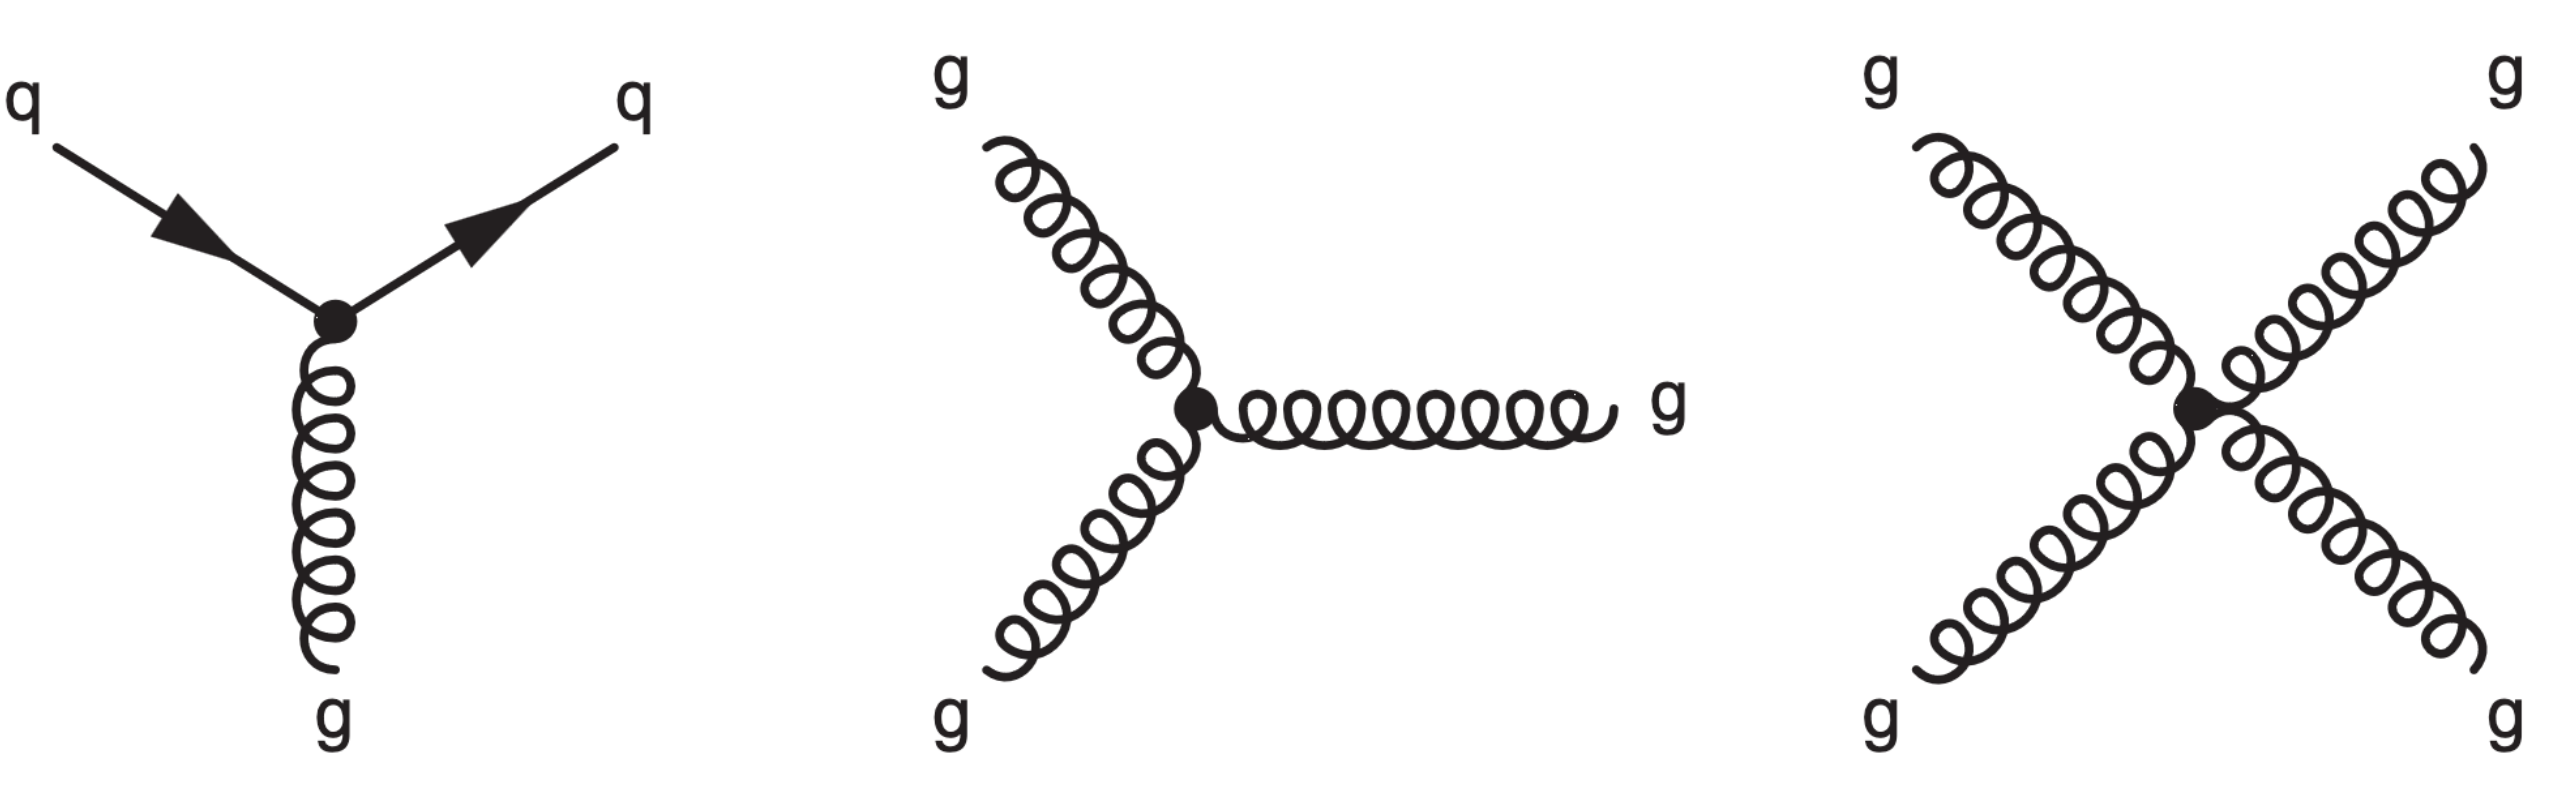
\includegraphics[width=0.8\textwidth]{gluon_gluon_interactions}
    \caption[]{(left) Quarks interacting with a gluon. (middle) triplet and (right) quartic self coupling of gluons. Adopted from \citep{thomson2013modern}.}
    \label{fig:qcd_vertices}
\end{figure}

\section{Renormalization}
\begin{figure}
    \centering
    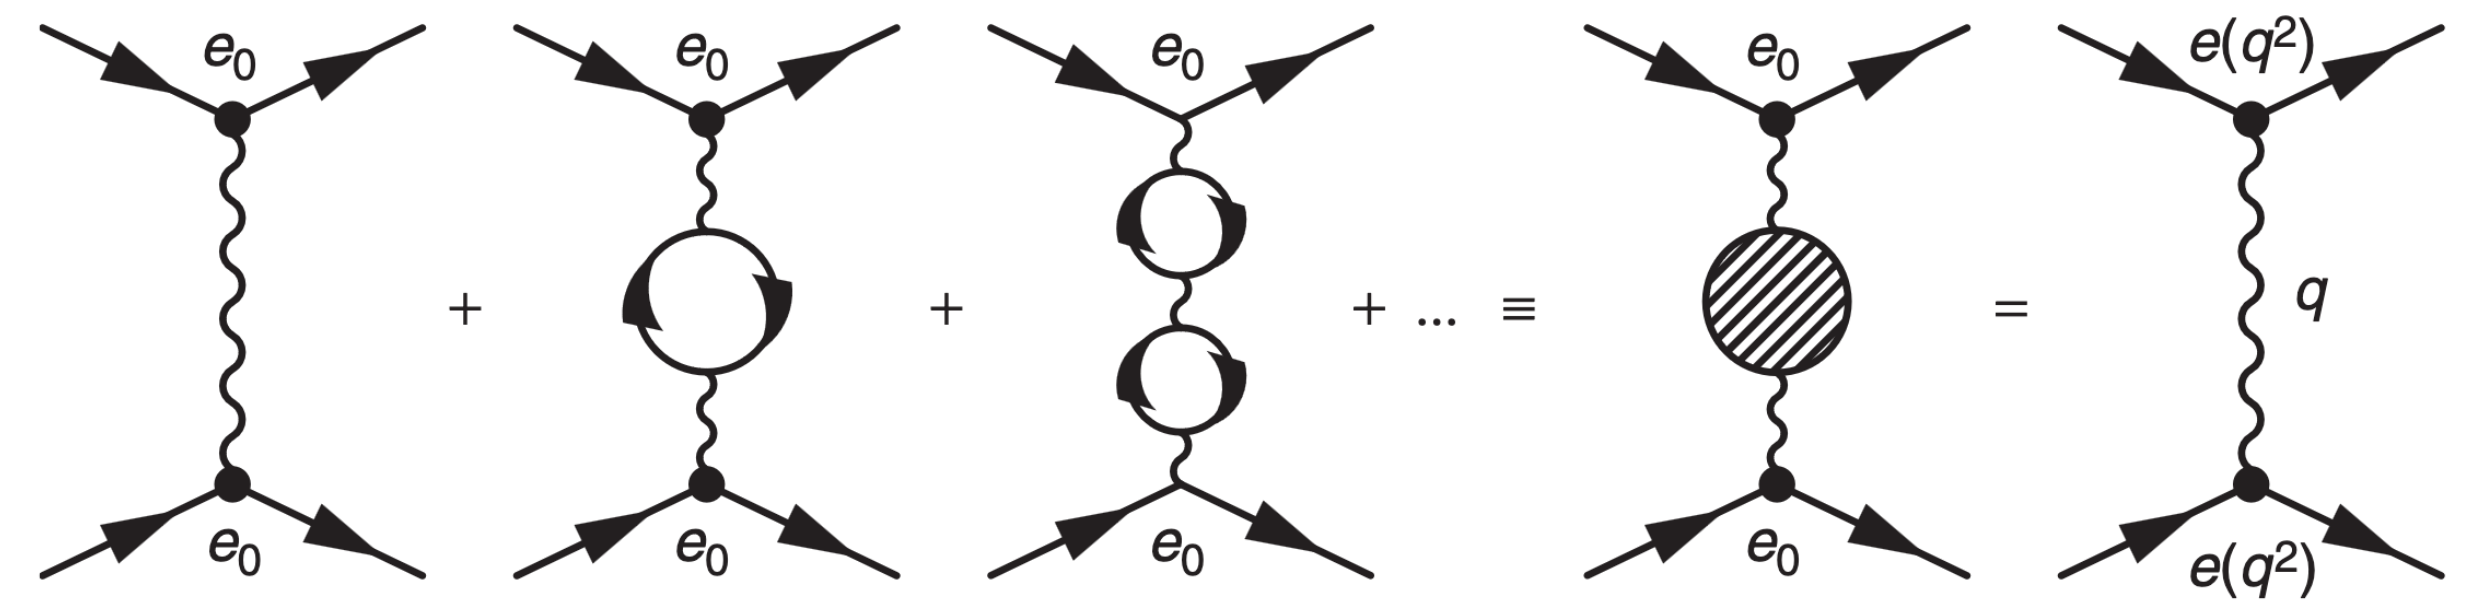
\includegraphics[width=1\textwidth]{qed_diagrams}
    \caption[]{Higher order loop corrections in \ac{qed} schematically treated as one effective diagram. Adopted from \citep{thomson2013modern}.}
    \label{fig:qed_diagrams}
\end{figure}
When trying to calculate amplitudes $\mathcal{M}$ of higher order diagrams in \ac{qed} like the second or third one in figure \ref{fig:qed_diagrams} it results in diverging integrals. These diagrams are also referred to as vacuum polarization as virtual particle-antiparticle pairs screen the actual charge of the electron $e_0$ like a dielectric medium in classical electrodynamics. The situation can be fixed by absorbing the appearing infinities into an effective charge/coupling $e(q^2)$ which is now a function of the squared four momentum $q^2$ at the virtual photon vertex shown schematically in figure \ref{fig:qed_diagrams}. For the the second diagram in figure \ref{fig:qed_diagrams} involving only one loop correction it can be shown that for some measured coupling $e(q^2=\mu^2)$ the actual coupling $e(q^2)$ follows a scaling behavior that holds if $q^2$ and $\mu^2$ are larger than the electron mass \citep{thomson2013modern}. The coupling constant is now a running coupling $e(q^2)$ and reads in terms of the fine structure constant $\alpha(q^2)=e^2(q^2)/4\pi$,
\begin{equation}
    \alpha(q^2)=
    \frac{\alpha(\mu^2)}
    {1-\alpha(\mu)\frac{1}{3\pi}
        \ln
        \left(\frac{q^2}{\mu^2}\right)}.
    \label{eq:qed_coupling}
\end{equation}
Therefore with increasing momentum transfer or closer approach in a collision the coupling at the virtual photon vertex increases as can be seen qualitatively in figure \ref{fig:renorm_scaling}(a).
\begin{figure}
    \centering
    \subfigure[]{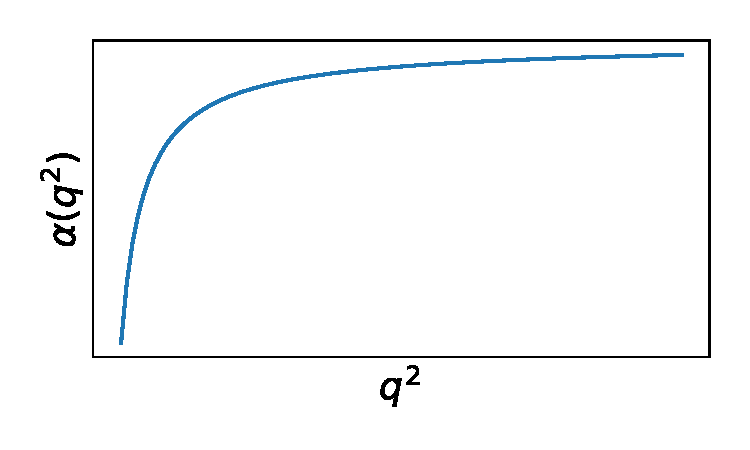
\includegraphics[width=.49\textwidth]{qed_scaling}}
    \subfigure[]{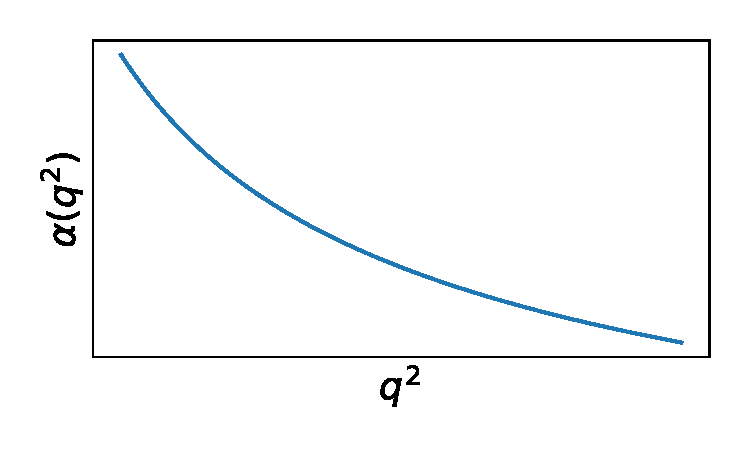
\includegraphics[width=.49\textwidth]{qcd_scaling}}
    \caption[]{Qualitative behavior of the running couplings for (\textbf{a}) \ac{qed} as of equation \ref{eq:qed_coupling} and (\textbf{b}) \ac{qcd} as of equation \ref{eq:qcd_coupling}.}
    \label{fig:renorm_scaling}
\end{figure}
\begin{figure}[H]
    \centering
    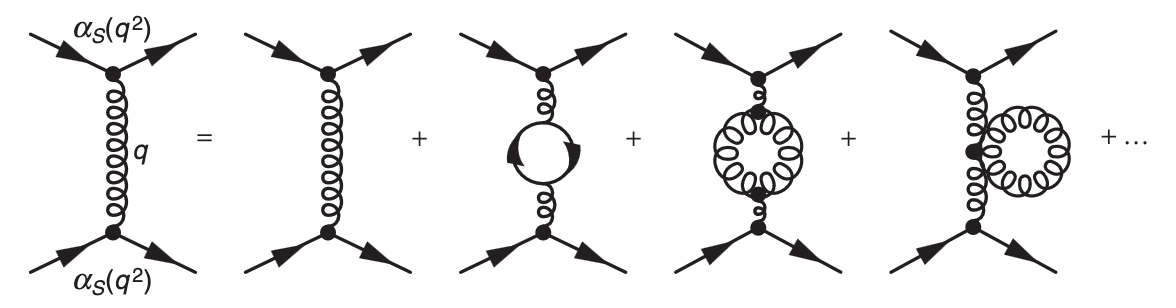
\includegraphics[width=1\textwidth]{qcd_diagrams}
    \caption[]{Some higher order loop corrections in \ac{qcd}. Adopted from \citep{thomson2013modern}.}
    \label{fig:qed_diagrams}
\end{figure}
Renormalization in \ac{qcd} can be derived similarly but also the quartic and triplet couplings exemplified in figure \ref{fig:qed_diagrams} need to be considered that result in a scaling for the strong coupling
\begin{equation}
    \alpha_S(q^2)=
    \frac{\alpha_S(\mu^2)}
    {1+B\alpha_S(\mu)
        \ln
        \left(\frac{q^2}{\mu^2}\right)}, \qquad \text{with } B=\frac{11N_c-2N_f}{12\pi}.
    \label{eq:qcd_coupling}
\end{equation}
For 3 color charges $N_c$ and 6 fermions $N_f$ in the \ac{sm}, $B$ is positive and the coupling becomes weaker for shorter scales or higher momentum transfer as can be seen in figure \ref{fig:renorm_scaling}(b).

The fine structure constant of \ac{qed} $\alpha(q^2\approx 0)\approx 1/137$ does not vary dramatically over the energy ranges of matter for particle physics as shown in figure \ref{fig:renorm_scaling_exp}(a).
\begin{figure}
    \centering
    \subfigure[]{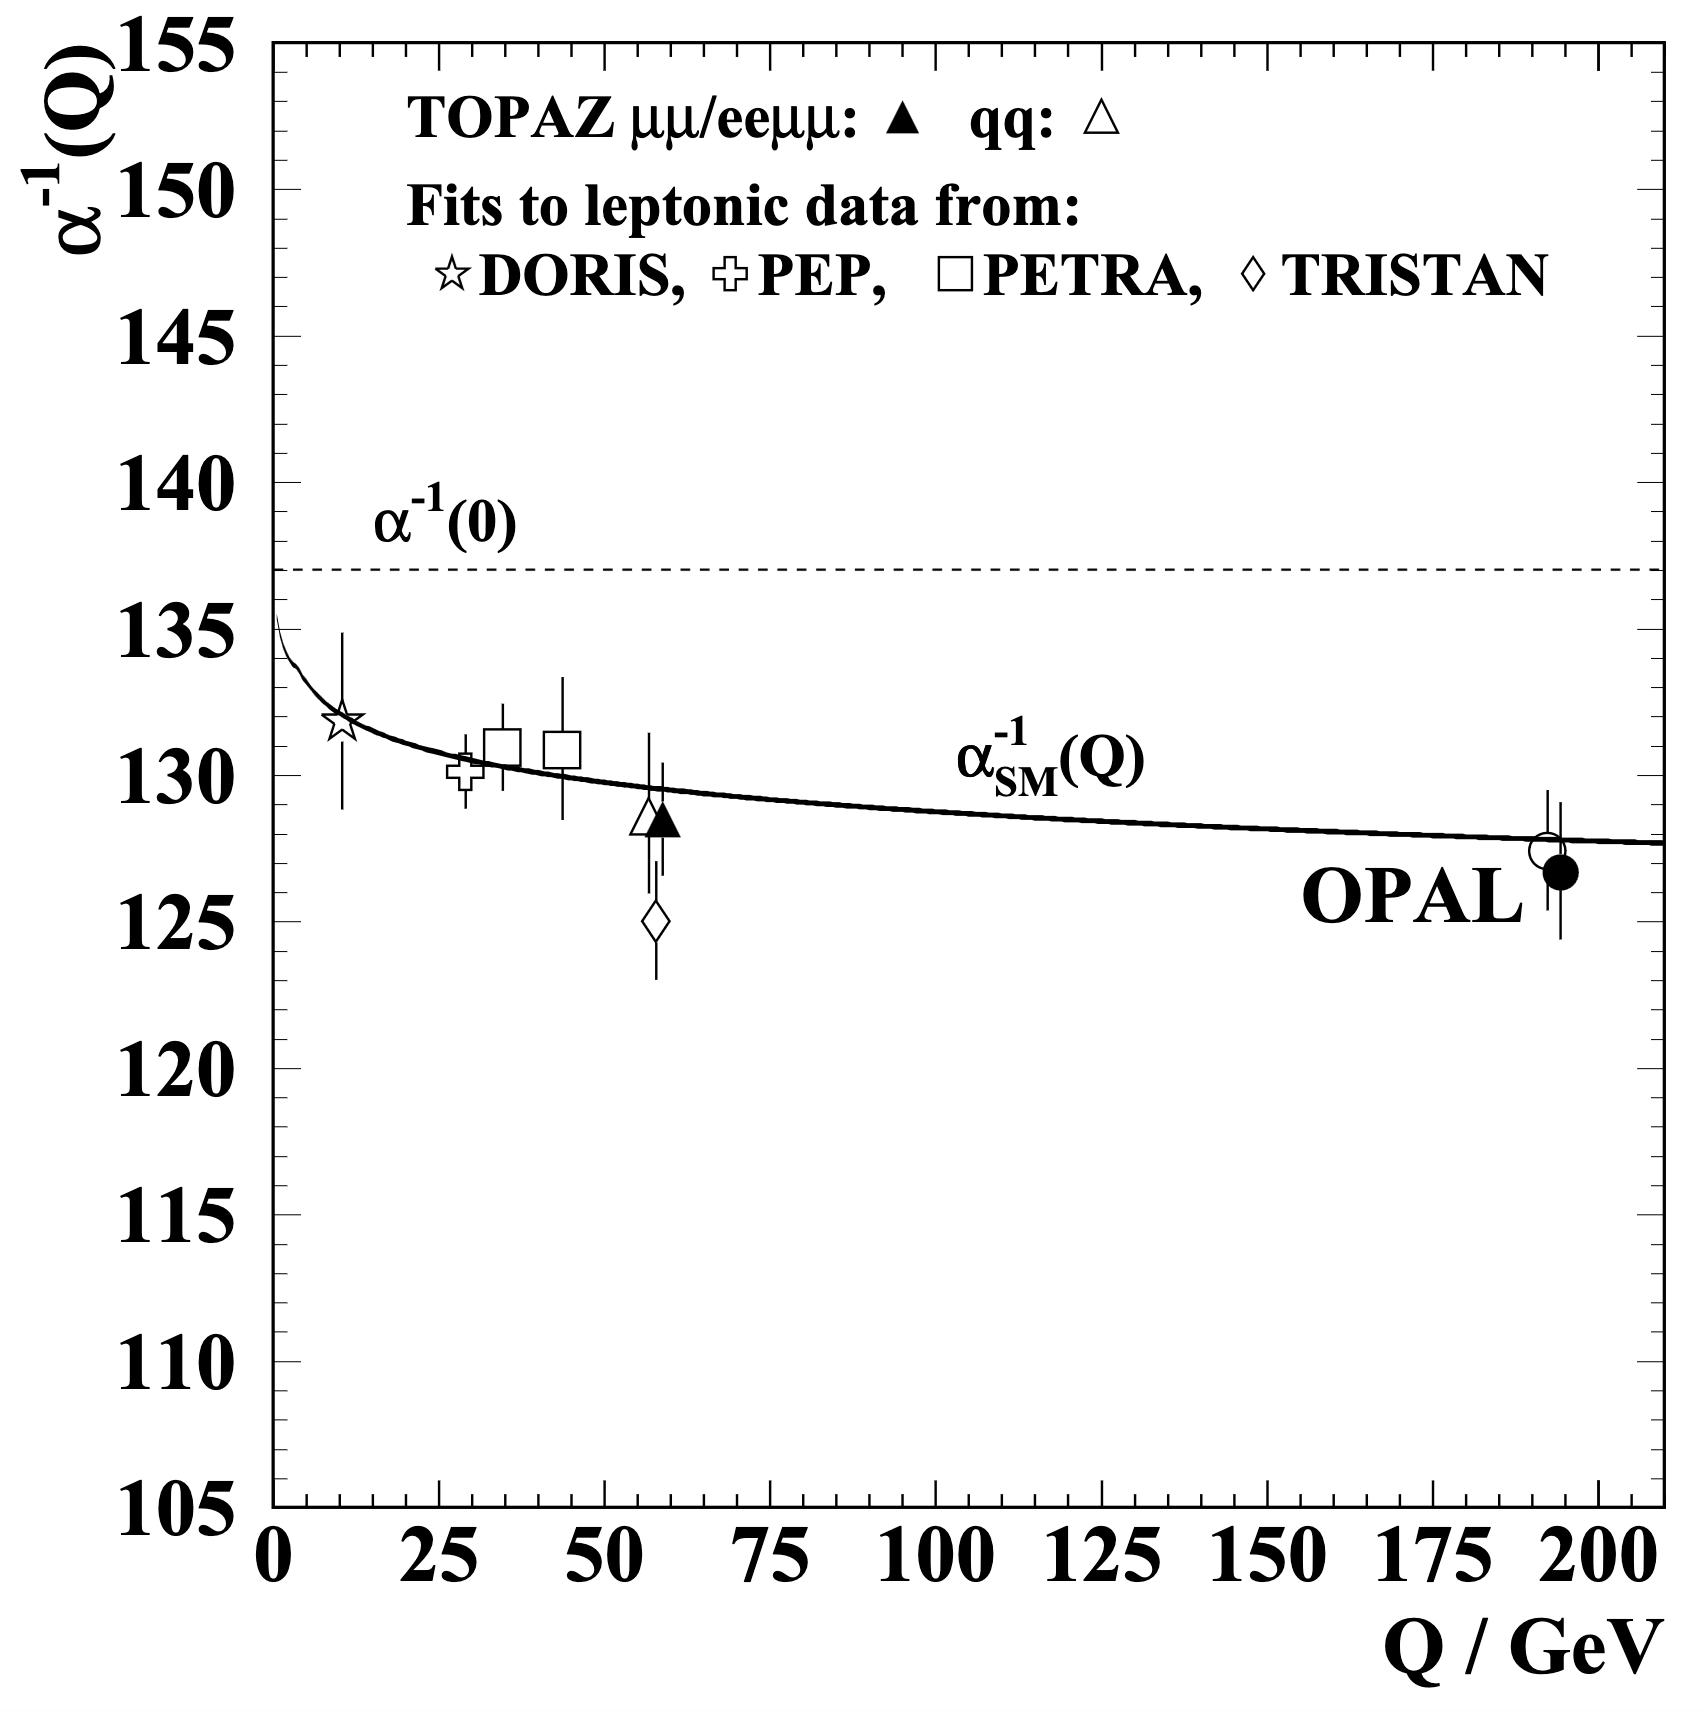
\includegraphics[width=.47\textwidth]{qed_scaling_experiment}}\hspace{5mm}
    \subfigure[]{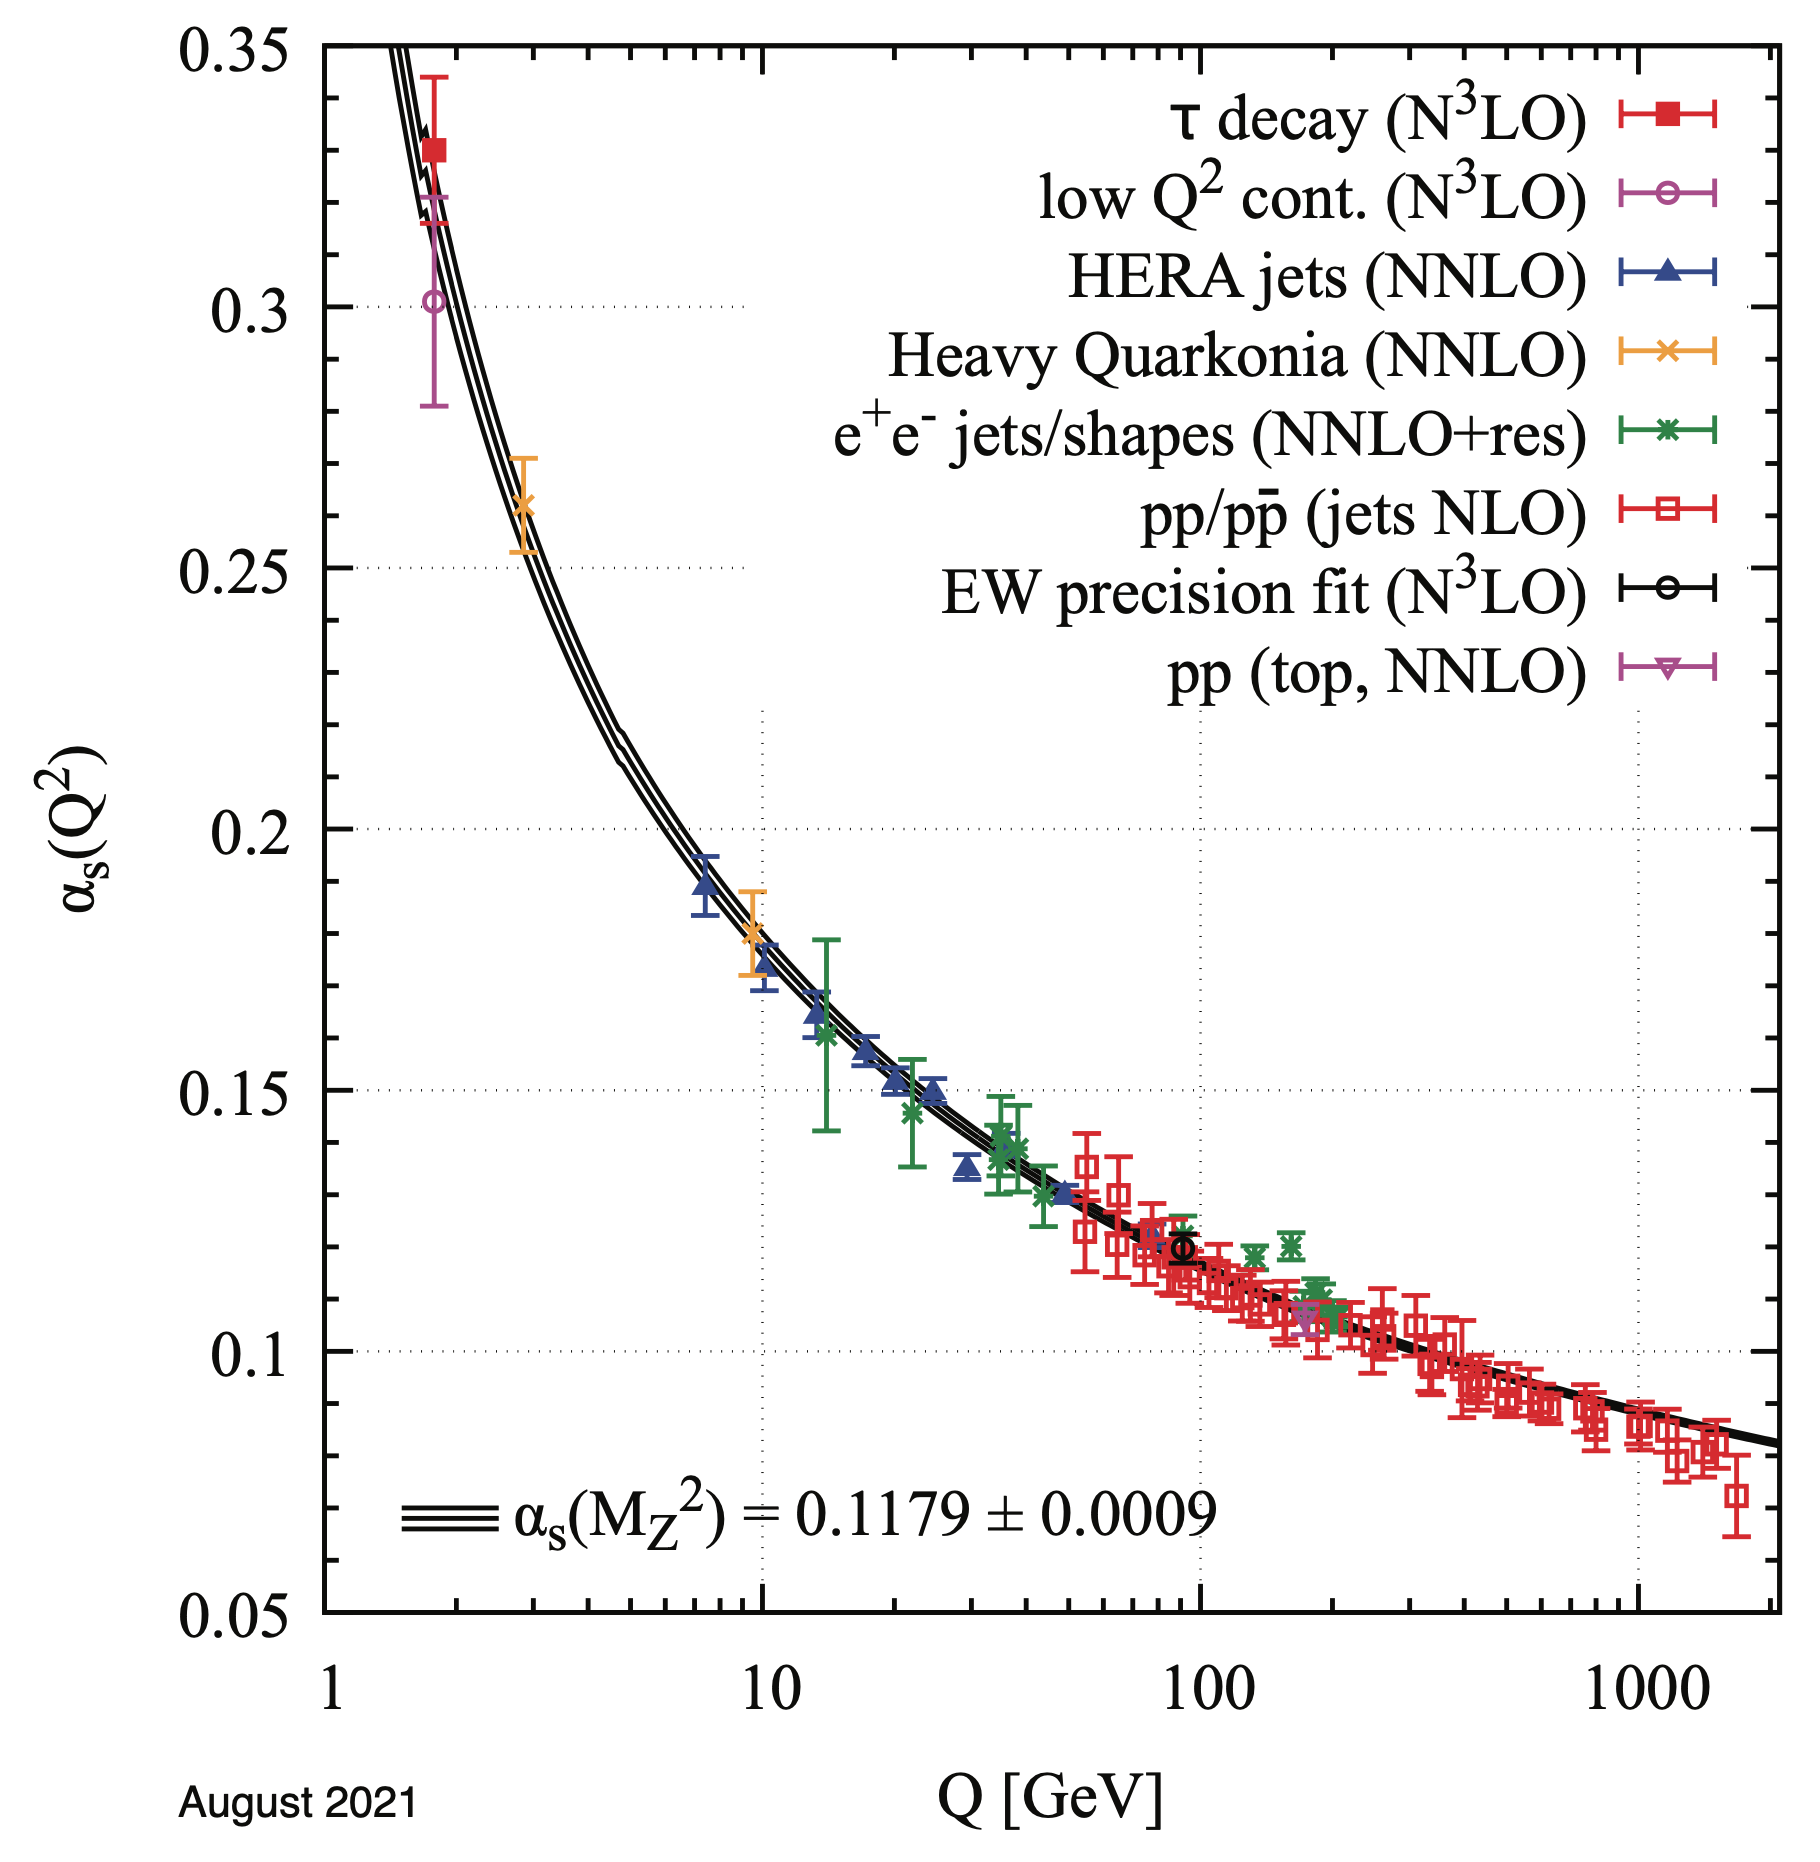
\includegraphics[width=.47\textwidth]{qcd_scaling_experiment}}
    \caption[]{Measurements of the running couplings for (\textbf{a}) \ac{qed} (note the inverted coupling on the y-axis) adopted from \citep{opal2004tests} and (\textbf{b}) \ac{qcd} adopted from \citep{particle2022review}.}
    \label{fig:renorm_scaling_exp}
\end{figure}
Most importantly the running coupling of \ac{qed} does not disturb the perturbation ansatz sketched out in section \ref{sec:qft} since $\alpha\ll1$. This is not the case for \ac{qcd} where $\alpha_S$ at $q\approx\SI{1}{GeV}$ is of $\mathcal{O}(1)$ and perturbation theory breaks down for calculations on bound hadronic states and latter processes in hadronization. While perturbation theory for \ac{qcd} remains valid for $\alpha_S\approx 0.1$ which corresponds to $q\approx \SI{100}{GeV}$ in basically all processes that are of interest at the \ac{lhc} higher order corrections must be considered in QCD calculations.

The behavior of the running coupling in \ac{qcd} is called asymptotic freedom, since the theory is free of asymptotics with increasing energy scale or decreasing distance. In turn, since the coupling increases with larger distances, this leads to color confinement, which means that colored particles can only be observed in bound states.

\section{Electroweak Unification}
The weak force can be added to the gauge invariant formalism with a $SU(2)$ symmetry and can be combined with the electromagnetic force so that both forces originate from one electroweak force by requiring a symmetry $SU(2)_L \otimes U(1)_Y$. The weak force couples to left handed chiral particle states only, e.g. for some fermion $\psi_L$. Fermions can be grouped by their characteristics into left handed doublets
\begin{equation}
    \begin{pmatrix}
        \nu_e \\ e
    \end{pmatrix}_L, \;
    \begin{pmatrix}
        \nu_\mu \\ \mu
    \end{pmatrix}_L, \;
    \begin{pmatrix}
        \nu_\tau \\ \tau
    \end{pmatrix}_L, \;
    \begin{pmatrix}
        u \\ d
    \end{pmatrix}_L, \;
    \begin{pmatrix}
        c \\ s
    \end{pmatrix}_L, \;
    \begin{pmatrix}
        t \\ b
    \end{pmatrix}_L, \;
    \label{eq:weak_doublets}
\end{equation}
with weak isospin $I=1/2$, with the third component $I_3=\pm1/2$ for the upper and lower doublet particle respectively, whereas the weak hypercharge $Y$ is associated to right handed singlets
\begin{equation}
    e_R    ,\quad \mu_R ,\quad    \tau_R ,\quad    u_R,\quad d_R ,\quad    c_R ,\quad s_R ,\quad    t_R ,\quad b_R,
\end{equation}
with $I=0$. The relation between the electric charge of the particle and these quantum numbers is governed by the Gell-Mann-Nishijima Formula $Q=I_3+Y/2$. The electroweak Lagrangian
\begin{equation}
    \mathcal{L}_\mathrm{EW} = \mathcal{L}_\mathrm{fermions}+\mathcal{L}_\mathrm{gauge}+\mathcal{L}_\mathrm{Higgs}+\mathcal{L}_\mathrm{Yukawa},
    \label{eq:L_EW}
\end{equation}
is then composed of four basic terms. Following the same steps as for \ac{qcd} and \ac{qed} the Lagrangian can be rendered gauge invariant by introducing a covariant derivative and gauge fields that are dictated by the group symmetry.

$SU(2)$ is generated through the three Pauli matrices $\bm{\sigma}$ requiring 3 vector gauge fields $W^a_\mu$, $a=\{1,2,3\}$ whereas the $U(1)$ symmetry of the vector gauge field $B_\mu$ is generated by the hypercharge $Y$. As before in order for the Lagrangian to be locally gauge invariant the new vector fields are massless. This gives the fermionic and gauge parts of the Lagrangian and will be explained below. The masses for the fermions and bosons can be incorporated via the Higgs mechanism that is described in section \ref{sec:higgs_mechanism} yielding the Higgs and Yukawa parts of the Lagrangian.


\subsubsection*{Fermion term}
To distinguish left- and right handed particle states the according spinors can be written as
\begin{equation}
    \psi_L=\frac{1-\gamma^5}{2}\psi, \quad \psi_R=\frac{1+\gamma^5}{2}\psi.
\end{equation}
These are not helicity eigenstates but rather $\psi_{L,R}$ become $\psi$, if $\psi$ has the corresponding helicity and vanish otherwise. The aforementioned doublets and singlets are then represented by
\begin{equation}
    \psi_L^j=
    \begin{pmatrix}
        \psi_{L+}^j \\ \psi_{L-}^j
    \end{pmatrix},
    \quad \psi_{R\xi}^j,
\end{equation}
with $j$ running over the doublets from equation \ref{eq:weak_doublets} and $\xi=+$ for u-type fermions and $\xi=-$ for d-type fermions.
The covariant derivative is
\begin{align}
    D_\mu^L & =\partial_\mu- i g_2 \frac{{\sigma}_a}{2}W_\mu^a+i g_1\frac{Y}{2}B_\mu, \label{eq:cov_diff_L} \\
    D_\mu^R & =\partial_\mu+ i g_1\frac{Y}{2}B_\mu,
\end{align}
with coupling $g_2$ and $g_1$ to the vector fields and $\sigma_a$ for the corresponding Pauli matrix, so that the fermionic part of the Lagrangian becomes
\begin{equation}
    \mathcal {L}_\text{fermions} = \sum_j\overline{\psi}^j_L i \gamma^\mu D_\mu^L\psi_L^j+\sum_{j,\xi}\overline{\psi}^j_{R\xi} i \gamma^\mu D_\mu^R\psi_{R\xi}^j.
    \label{eq:L_fermion}
\end{equation}

\subsubsection*{Gauge term}
The gauge field self interaction terms are
\begin{align}
    W_{\mu\nu}^a & =\partial_\mu W_\nu^a-\partial_\nu W_\mu^a+g_2\epsilon_{abc}W_\mu^b W_\nu^c, \\
    B_{\mu\nu}   & =\partial_\mu B_\nu-\partial_\nu B_\mu,
\end{align}
with $g_2$ the weak coupling constant and $\epsilon_{abc}$ the totally asymmetric Levi-Civita tensor yielding the gauge field part of the Lagrangian
\begin{equation}
    \mathcal {L}_\text{gauge} = -\frac{1}{4} W_{\mu\nu}^a W^{\mu\nu,a} - \frac{1}{4}B_{\mu\nu}B^{\mu\nu}.
\end{equation}
At this point the gauge fields $W^a_\mu$ are still massless because they would break the gauge symmetry. Masses can be incorporated into the Lagrangian with the Higgs mechanism explained in section \ref{sec:higgs_mechanism}.

\section{Higgs mechanism}\label{sec:higgs_mechanism}

In the previous sections, it was shown that the principle of local gauge invariance applied to the free Dirac Lagrangian can generate all the dynamics for a given interaction. However, this assumes that the accompanying gauge boson vector fields are massless, which is not the case for the weak interactions. The Higgs mechanism adds a field to the Lagrangian that provides mass terms for the vector bosons and fermions while preserving the principle of local gauge invariance. The simplest way to achieve this is to introduce a complex scalar field
\begin{equation}
    \phi (x)=\frac{1}{\sqrt{2}}(\phi_1(x)+i\phi_2(x))
\end{equation}
so that a Lagrangian with a kinetic term $T(\phi)$ and a potential $V(\phi)$ with parameters $\mu$ and $\lambda$ can be constructed as
\begin{equation}
    \mathcal{L}=T(\phi)-V(\phi)=
    \left[\left(\partial_\mu\phi\right)^* (\partial^\mu\phi)\right]
    -\left[
        -\mu^2(\phi^*\phi)+\lambda(\phi^*\phi)^2
        \right].
\end{equation}
To make this Lagrangian locally gauge invariant the transformation steps from section \ref{sec:qed} on \ac{qed} can be followed. Again by replacing the derivative with the covariant derivative with some vector field $B_\mu$ and coupling $g$
\begin{equation}
    \partial_\mu \rightarrow D_\mu = \partial_\mu + ig B_\mu.
\end{equation}
The resulting Lagrangian can be made locally gauge invariant with the transformations
\begin{align}
    \phi(x)  & \rightarrow  e^{-i \alpha(x)}\phi(x),                      \\
    B_\mu(x) & \xrightarrow{} B_\mu(x) -\partial_\mu\alpha(x).
\end{align}

The lowest energy state of a free field theory is the vacuum state and therefore its eigenvalue $v$ is also called \ac{vev}. It is the one that minimizes the potential $V(\phi)$
\begin{equation}
    v =
    \begin{cases}
        0                                                     & \lambda>0, \mu^2<0 \\
        \sqrt{\phi_1^2+\phi_2^2}=\sqrt{\frac{\mu^2}{\lambda}} & \lambda>0, \mu^2>0
    \end{cases}
\end{equation}
and is either 0 or forms an infinite set of minima as illustrated in figure \ref{fig:higgs_potential} by the dashed circle.
\begin{figure}
    \centering
    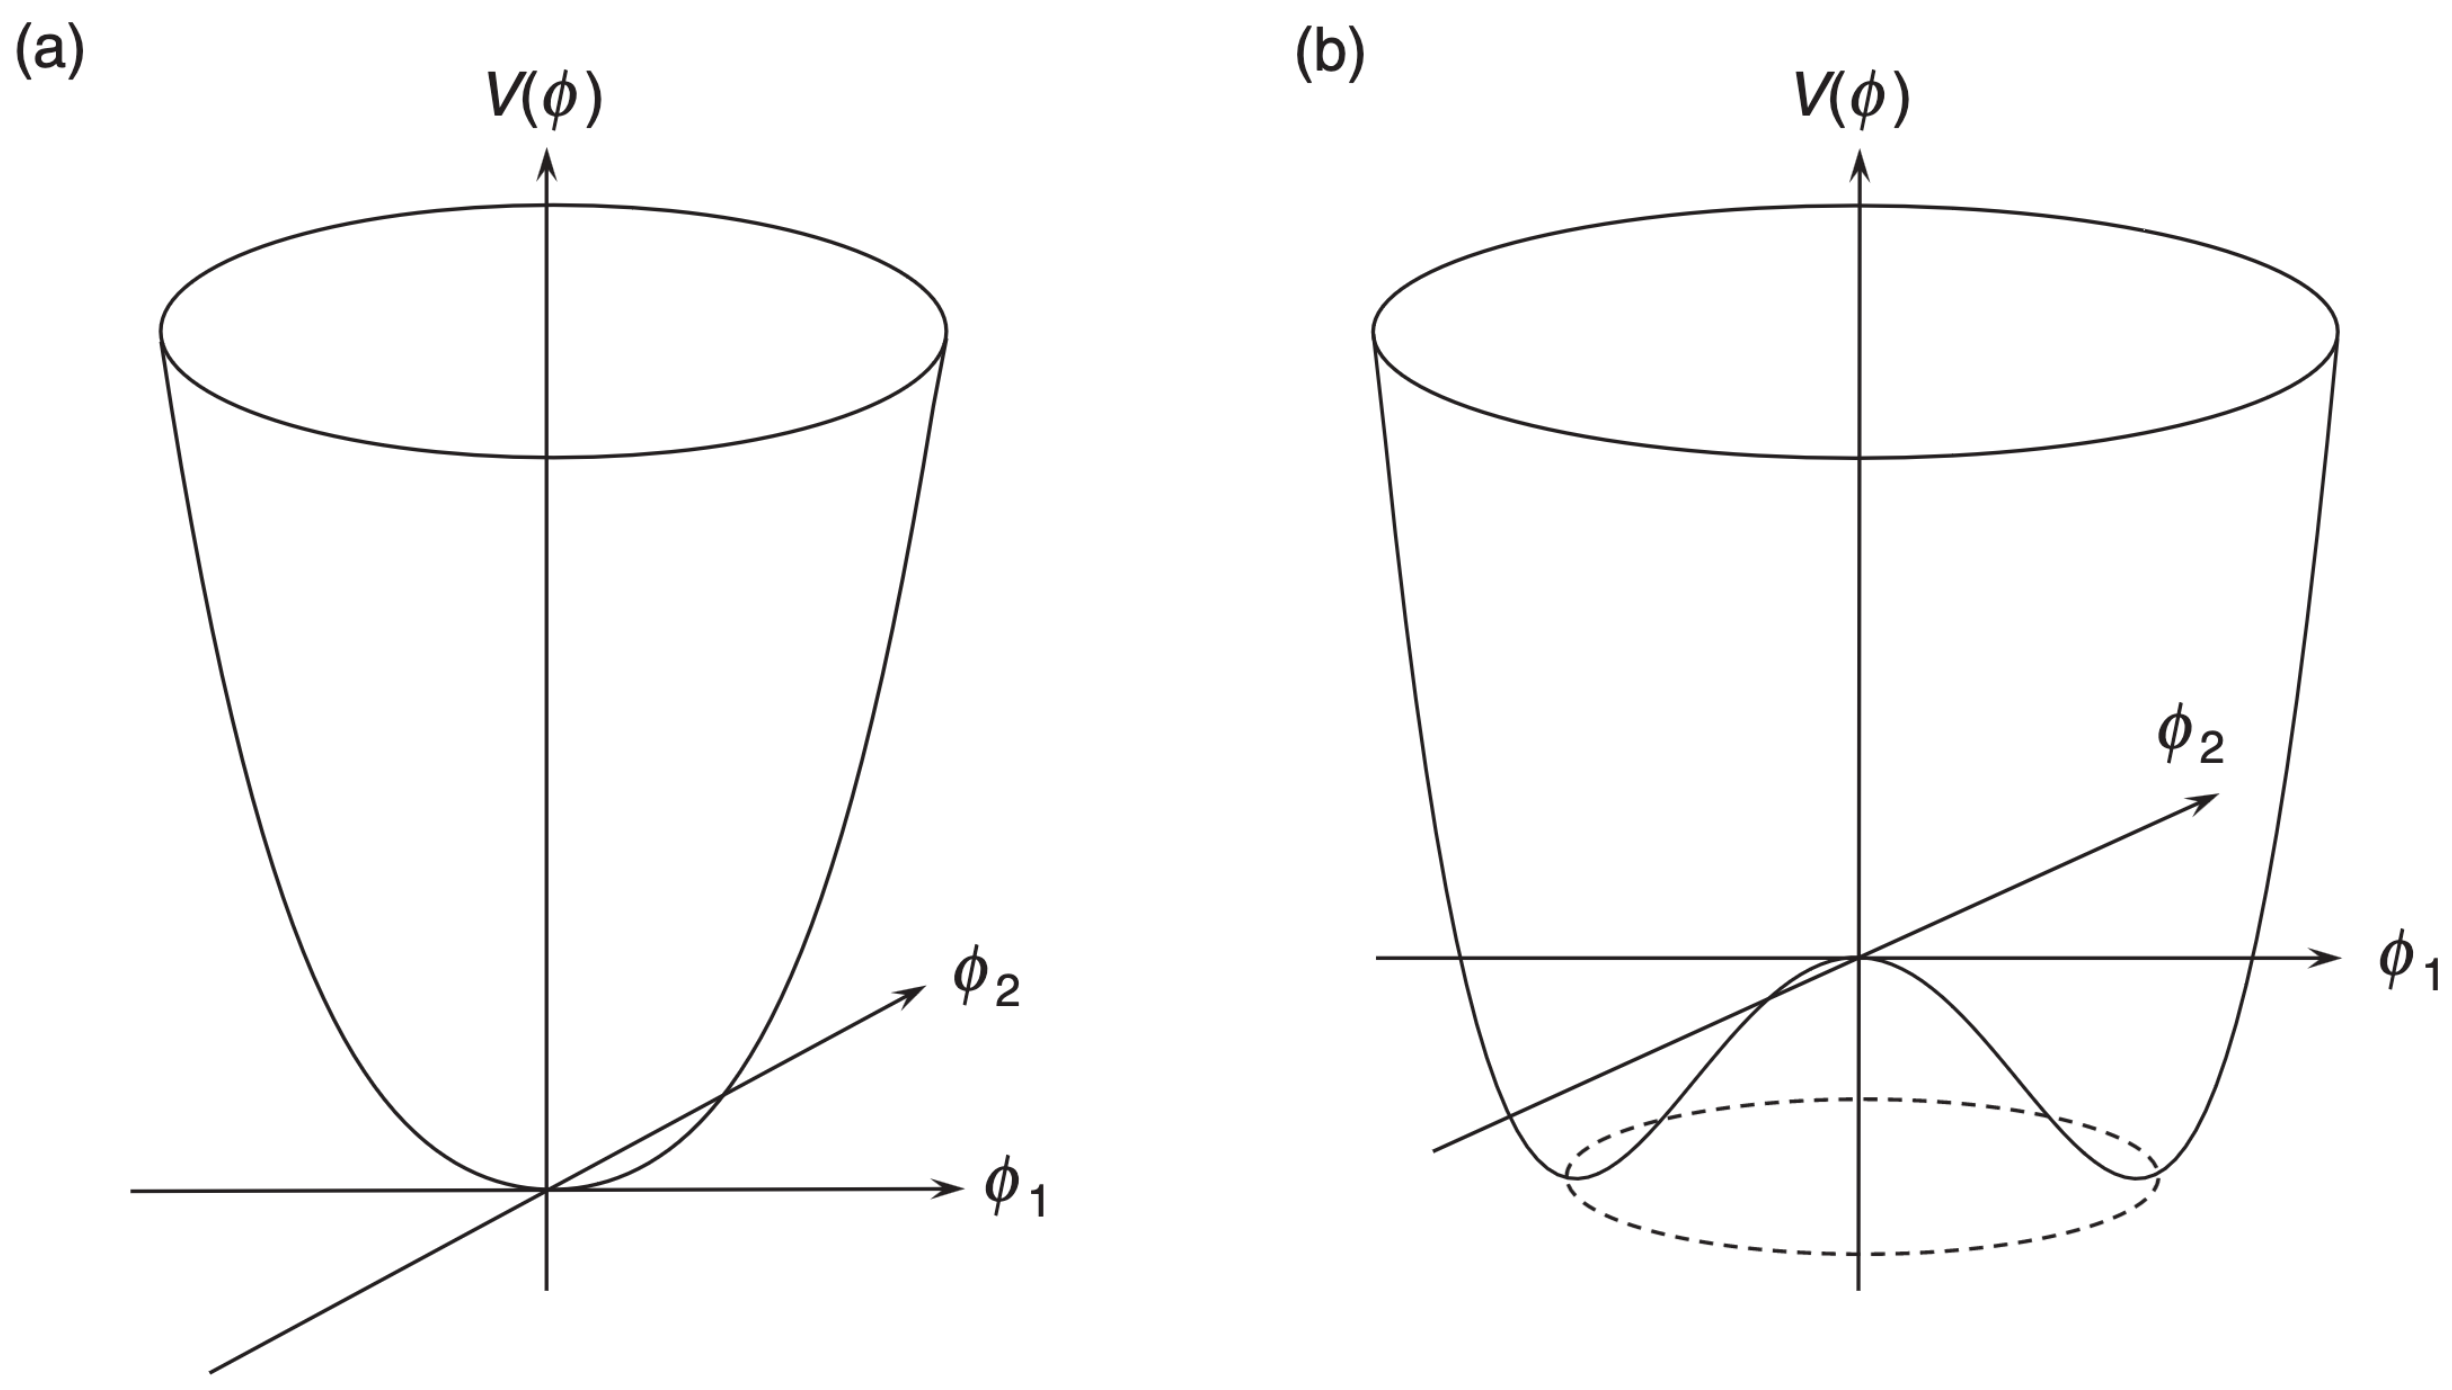
\includegraphics[width=.8\textwidth]{higgs_potential}
    \caption[]{Potential $V(\phi)$ (a) for $\lambda>0$ and $\mu^2<0$ and (b) for values $\lambda>0$ and $\mu^2>0$. Adopted from \citep{thomson2013modern}.}
    \label{fig:higgs_potential}
\end{figure}

The perturbation ansatz sketched out in section \ref{sec:qft} considers perturbations around the ground state. Thus for the ansatz to work with the $\mu^2>0$ case new field variables $eta(x)$ and $\xi$ can be introduced so they can be perturbed about the ground state
\begin{equation}
    \phi_1(x)=v+\eta(x),\quad \phi_2=\xi.
\end{equation}
Therefore the physical vacuum state spontaneously breaks the symmetry of the Lagrangian. Plugging this into the Lagrangian already gives a mass term to a vector boson. The predictions of the Lagrangian do not depend on the choice of the gauge. When choosing it to be $\alpha(x)=-\xi(x)/(gv)$, also called unitary guage, the $\xi$ field can be eliminated entirely so the complex scalar field only depends on the \ac{vev} and $\eta(x)$ becomes the physical Higgs field $h(x)$
\begin{equation}
    \phi(x)=\frac{1}{\sqrt{2}}(v+\eta(x)+i\xi(x)) 
    \stackrel{\text{unitary gauge}}{=} 
    \frac{1}{\sqrt{2}}(v+h(x)).
\end{equation}
The final Lagrangian then is
so the final Lagrangian becomes


\red{ gauge from griffiths better, beacuse exact}



\begin{figure}
    \centering
    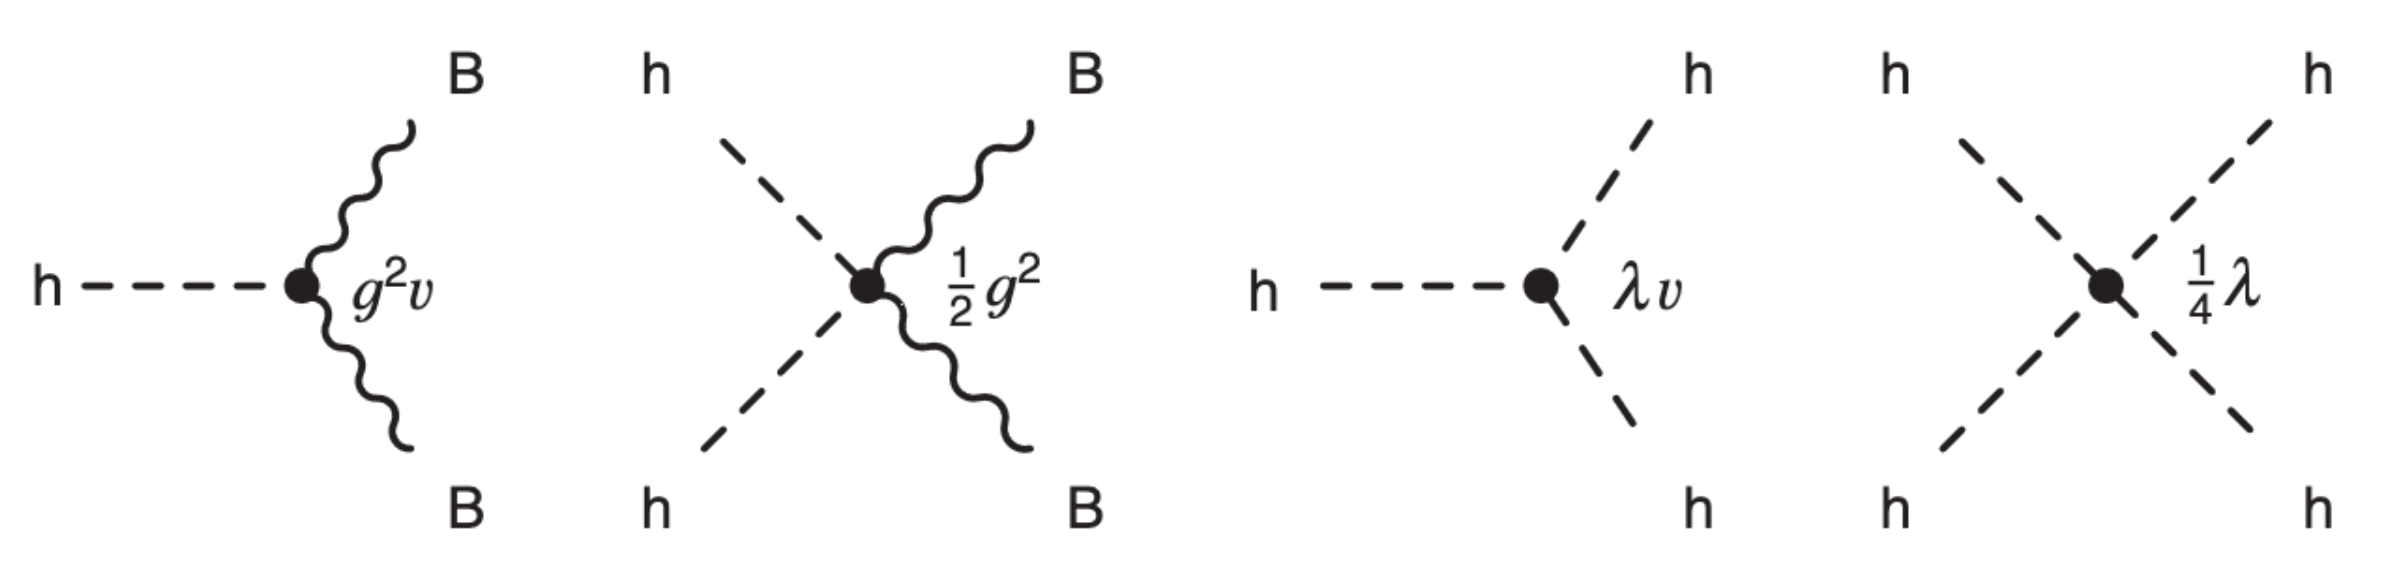
\includegraphics[width=.8\textwidth]{higgs_couplings}
    \caption[]{Higgs interaction terms arising from a local the Higgs mechanism for a local $U(1)$ gauge symmetry. Adopted from \citep{thomson2013modern}.}
    \label{fig:higgs_couplings}
\end{figure}







physical predications of the theory are unchanged by
the gauge transformation


move L into vev for perturbation ansatz, also needed to get mass term? true symmetry concealed by picking a particular ground state. both L represent the same physical system as the equations of motion



show L

choose a particular gauge
























breaks down the $SU(2)_L \otimes U(1)_Y$ symmetry while maintaining the electromagnetic $U(1)_{EM}$ symmetry which is also called \ac{ewsb} and allows mass terms for the gauge bosons of the electroweak Lagrangian. The \ac{sm} Higgs field is a single isospin doublet of complex scalar fields
\begin{equation}
    \phi(x)=
    \begin{pmatrix}
        \phi^+(x) \\
        \phi^0(x)
    \end{pmatrix}
    =
    \begin{pmatrix}
        \phi_1 (x)+i \phi_2 (x) \\
        \phi_3 (x)+i \phi_4 (x),
    \end{pmatrix}
\end{equation}
with hyperchage $Y=1$ so that the covariant derivative from equation \ref{eq:cov_diff_L} reads
\begin{equation}
    D_\mu=\partial_\mu- i g_2\frac{{\sigma}_a}{2}W_\mu^a+ i\frac{g_1}{2}B_\mu.
\end{equation}
\subsubsection*{Higgs term}
The Higgs term for the electroweak Lagrangian in equation \ref{eq:L_EW} then is
\begin{equation}
    \mathcal{L}_\text{Higgs}= \left(D_\mu\phi\right)^\dagger (D^\mu\phi)-V(\phi),
    \label{eq:L_higgs}
\end{equation}
with the Higgs potential
\begin{equation}
    V(\phi) = -\mu^2\phi^\dagger\phi+\frac{\lambda}{4}\left(\phi^\dagger\phi\right)^2.
    \label{eq:Higgs_V}
\end{equation}

the choice is such that


containing parameters $\mu$ for the Higgs mass and $\lambda$ for the strength of the Higgs fields self-interaction.



\subsubsection*{Yukawa term}

